
\chapter{Implementation}
\label{ch:chapter03}

This chapter outlines the development process of the \acs{PoC} / \acs{FPGA} Verification Platform for this thesis. All components, including hardware designs, programmable logic modules, signal generators, analysis tools, and software, were developed from first principles. No pre-existing verification frameworks, \acs{IP} extensions, or platform structures were available for adaptation. Each functional block discussed in the following sections, ranging from digital stimulus generation to closed-loop signal evaluation, represents original work created specifically for this proof-of-concept. The chapter provides a comprehensive account of the implementation process prior to evaluating system performance.

\section{Current Sense Verification}
\label{sec:Implementation:Current_Sense_Verification}

Within the Current Sense verification system, the Current Sense path functions as a black box. The \acs{ADC} on the control board receives analog inputs, either static or dynamic, corresponding to each motor phase as mentioned in the section \ref{sec:Conecpt:UnderstandingDUTs:CurrentSensepath}. The DAC80508 generates these analog signals. A high-level block diagram of the Current Sense Verification Closed-Loop architecture is provided in the figure \ref{fig:Implementation:CurrentSenseverification_BD}.

The system comprises three motor phases (U, V, and W) and supports two types of verification tests: static and dynamic. Accordingly, six control commands are defined.

\begin{enumerate}
	\item phu\_s\_a1 – Phase U Static Test Axis 1
	\item phv\_s\_a1 – Phase V Static Test Axis 1
	\item phw\_s\_a1 – Phase W Static Test Axis 1
	\item phu\_d\_a1 – Phase U Dynamic Test Axis 1
	\item phv\_d\_a1 – Phase V Dynamic Test Axis 1
	\item phw\_d\_a1 – Phase W Dynamic Test Axis 1
\end{enumerate}

Each control command specifies the phase under test and the verification type (static or dynamic). These commands are transmitted to the control board, where the test\_fsm module interprets the command and generates the corresponding feedback.

The \acs{PS} \acs{UART} interface on the Enclustra Mercury XU5 \acs{SoC} receives and parses the control commands. The relevant data is transferred to the \acs{PL} through the \acs{AXI} \acs{GPIO} interface. A custom MUX module processes the \acs{AXI} \acs{GPIO} inputs and handles \acs{DAC} initialization and configuration before data transmission.

\begin{itemize}
	\item For static verification, a single 16-bit value is written to the selected \acs{DAC} to emulate a constant analog signal.
	\item For dynamic verification, a 16-bit sine wave lut is written to the \acs{DAC} to emulate an analog sinusoidal waveform representative of motor feedback.
\end{itemize}

Three of the eight available \acs{DAC} channels on the DAC80508 evaluation board are used, each corresponding to one motor phase (U, V, and W). The appropriate \acs{DAC} channel is selected and updated with the required data based on the received command. 

\begin{figure}[t]
	\centering
	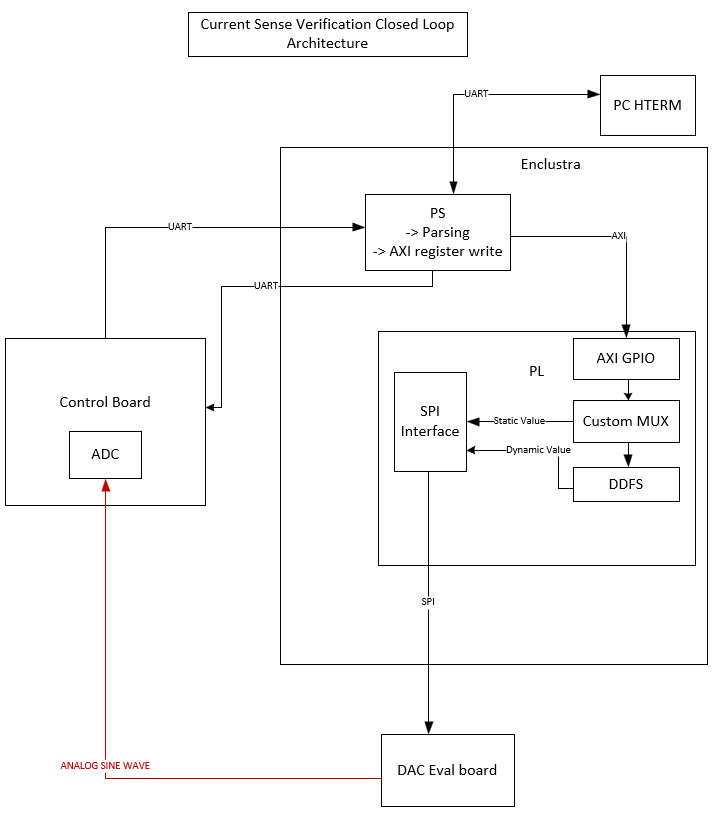
\includegraphics[width=0.70\textwidth]{gfx/diagrams/Current_Sense_Verification_Block_Design.png}
	\caption{Block Design of the Current Sense Verification}
	\label{fig:Implementation:CurrentSenseverification_BD}
\end{figure}

The Direct Digital Frequency Synthesis (\acs{DDFS}) module generates digital sine wave samples for dynamic verification. These samples are transmitted to the \acs{DAC} through an \acs{SPI} interface module. The \acs{ADC} on the control board measures the resulting analog output and, according to the test configuration, sends feedback to the Enclustra board via a secondary \acs{UART} interface.

During static tests, a single 12-bit \acs{ADC} value is returned. For dynamic tests, a \acs{FIFO} containing 2048 12-bit samples is transmitted. The \acs{PS} then performs the following verification steps.

\begin{itemize}
	\item In static tests, the received 12-bit \acs{ADC} value is compared with the corresponding 16-bit reference value transmitted from the Enclustra board.
	\item In dynamic tests, a \acs{FFT} is performed on the received 12-bit \acs{FIFO} data to verify the frequency content. If the \acs{FFT} result confirms the expected 1 kHz sine wave, the dynamic response is considered valid.
\end{itemize}

In a nutshell, to facilitate Current Sense Verification, the system interprets user commands and transmits the appropriate data to the \acs{DAC} channels. A dedicated Custom MUX module manages this process, acting as the interface between \acs{PS}-generated control signals and the \acs{DAC} configuration logic. The following section details the design and operation of this module.

\subsection{Custom MUX algorithmn}
\label{sec:Implementation:Custom_MUX_algorithmn}

The Command Parser, implemented in the \acs{PS}, writes the relevant data parsed from the control commands to the \acs{AXI} \acs{GPIO}. This data is then transferred to the Custom MUX module within the \acs{FPGA}, which configures the \acs{DAC} on the DAC80508 evaluation board. 

A state machine (figure~\ref{fig:Implementation:CurrentMUX}) is implemented to transmit the configuration command \textbf{0x30100} to the DAC80508 device. By default, the evaluation board utilizes a 2.5 V internal reference, however, an external reference may be used by disabling the internal reference via the CONFIG register \cite{TI_DAC80508}.

The \acs{DAC} requires a 24-bit hexadecimal command format. The first nibble indicates the operation type, with ‘0’ representing a read and ‘1’ representing a write. The second nibble specifies the register address, while the remaining 16 bits contain the data to be written or read. The command \textbf{0x30100} is sent to the CONFIG register (see Table \ref{table:Concept_and_Modeling:CONFIG_REG}) to power down the internal reference and enable an external 3.3 V reference source. In the following state, this configuration is verified by issuing the command \textbf{0x13000}, which allows the value to be read back through the MISO lines as confirmation.

%\begin{figure}[H]
%	\centering
%	\hspace{30cm} % adjust value: 0.5cm, 1cm, etc.
%	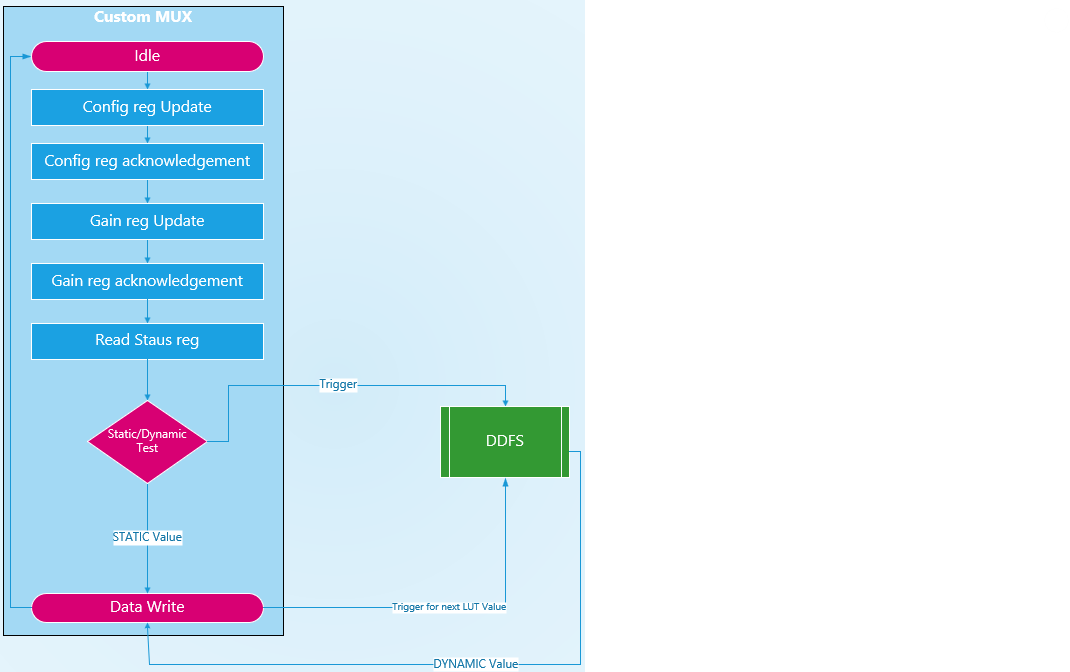
\includegraphics[width=0.80\textwidth, height=0.60\textwidth]{gfx/diagrams/Custom_MUX_Algorithmn.png}
%	\caption{Current MUX algorithmn}
%	\label{fig:Implementation:CurrentMUX}
%\end{figure}

Similarly, the Gain register is updated with the command \textbf{0x401FF}, configuring the \acs{DAC} so that the output gain is doubled and the reference voltage is internally divided by two (see Table \ref{table:Concept_and_Modeling:GAIN_Reg}). Depending on the control command, if static verification, a certain static Value is written to a \acs{DAC} register, if dynamic Verification, the \acs{DDFS} is triggered which starts to generate digital sine wave from a \acs{LUT} of 16 bit 1024 samples. The system executes one of two actions depending on the control command.

\begin{figure}[H]
	\centering
	\makebox[1.35\textwidth][1]{% 1.2 moves it right; increase/decrease as needed
		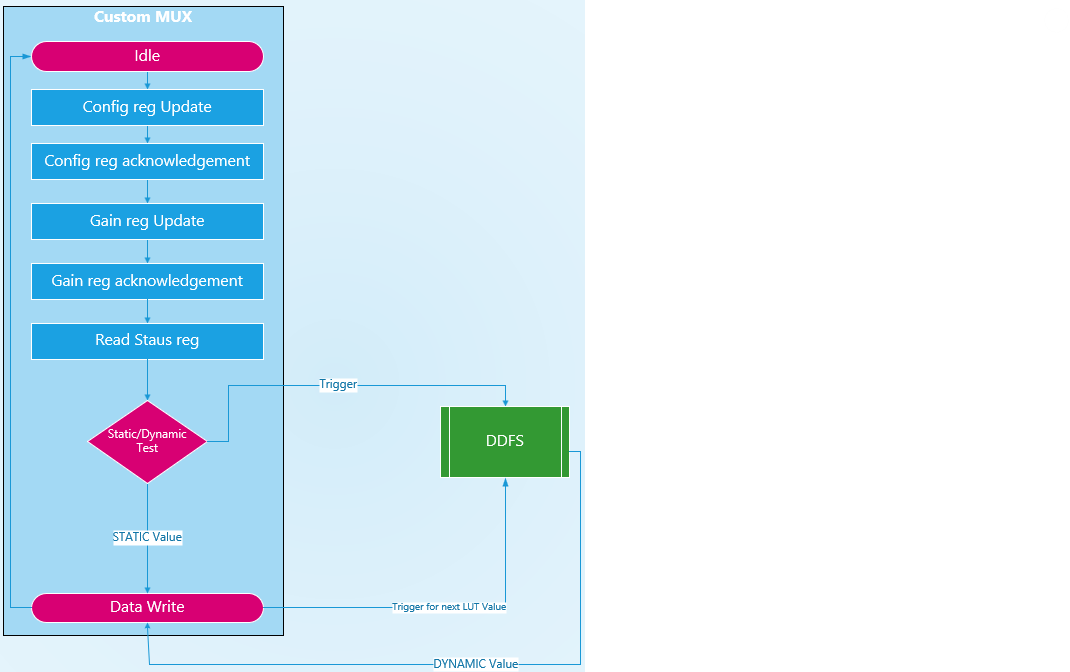
\includegraphics[width=0.80\textwidth, height=0.55\textwidth]{gfx/diagrams/Custom_MUX_Algorithmn.png}
	}
	\caption{Current MUX algorithm}
	\label{fig:Implementation:CurrentMUX}
\end{figure}

The Custom MUX selects the verification method, while generating dynamic test signals requires a precise digital waveform source. For this purpose, the system incorporates a Direct Digital Frequency Synthesis module that produces high-resolution sine waves. The following subsection details the \acs{DDFS} architecture, configuration parameters, and the process for generating the 1 kHz test signal.

\subsection{Direct Digital Frequency Synthesis}
\label{sec:Implementation:DDFS}

Direct Digital Frequency Synthesis is a widely recognized technique for generating sinusoidal signals in applications that require high frequency resolution, rapid frequency and phase transitions, and high spectral purity. \acs{DDFS} systems generate periodic, discrete-time waveforms at specified frequencies. Although the output waveform is typically a sine wave, \acs{DDFS} can also produce saw-tooth, triangle, square, or other periodic waveforms. The primary components of a \acs{DDFS} system are illustrated in Figure \ref{fig:Implementation:DDFS}.

\begin{figure}[htbp]
	\centering
	
\includegraphics[width=0.80\textwidth]{gfx/diagrams/DDFS.png}
	\caption{Direct Digital frequency Synthesis}
	\label{fig:Implementation:DDFS}
\end{figure}

\begin{itemize}
	\item \textbf{Time Base Generation} $\rightarrow$ The time-base module receives a 192 MHz system clock generated by the clocking wizard from a 100 MHz external oscillator. This module periodically enables the phase accumulator, allowing the \acs{DDFS} to output a sine wave at the specified frequency. The counter increments with each clock cycle and generates an enable pulse when it reaches a predefined threshold.
	
	\begin{lstlisting}
 	time_base_counter : process(clk, rst_n)
	begin
		if rising_edge(clk) then
			if rst_n = '0' then
				time_base <= (others => '0');
			else
				if ddfs_start = '1' then
					if time_base = parameter - 1 then
						time_base <= (others => '0');
					else
						time_base <= time_base + "1";
					end if;
				end if;
			end if;
		end if;       	
	end process time_base_counter;
	\end{lstlisting}
	
	\item \textbf{Phase Accumulator} $\rightarrow$ The phase accumulator generates the phase angle used to index into the sine look-up table. By adding the frequency-tuning word (FTW) at each enable pulse it determines both the output frequency and phase resolution.
	
	\begin{lstlisting}
	phase_acc_stimulus : process(clk) 
	begin
		if rising_edge(clk) then
			if rst_n = '0' then
				q_reg <= (others => '0');
			elsif enable = '1' then
				q_reg <= q_reg + unsigned(ftw);
			end if;
		end if;
	end process phase_acc_stimulus;
	\end{lstlisting}
	
	\item \textbf{Sine Wave \acs{LUT}} $\rightarrow$ The \acs{LUT} translates the accumulated phase value into a corresponding sine amplitude. It consists of 1024 samples, each 16 bits wide, representing a complete 360° sine wave.
\end{itemize}

A system clock frequency of 192 MHz is selected for the verification path. The goal is to synthesize a 1 kHz sine wave using the direct \acs{DDFS}. This target frequency is chosen based on the current verification setup (see Section \ref{sec:intro:ProblemStatement}), in which the motor drives are capable of generating phase-current feedback signals at 500–800 Hz. To achieve a 1 kHz output, the time-base generation module must trigger the phase accumulator once every 192 clock cycles. Assuming the use of 1,000 \acs{LUT} samples with 16-bit amplitude resolution, the output frequency can be calculated as follows:

\begin{align*}
	\frac{192 \times 10^6}{192 (Time base)} &= 10^6 \\
	&= \frac{10^6}{1000 (\acs{LUT} Samples)} \\
	&= 1\ KHz
\end{align*}

However, selecting 1,000 samples necessitates a 10-bit phase accumulator, which inherently provides 1,024 addressable entries. Because the phase accumulator directly indexes the sine \acs{LUT}, the table size must be expanded to 1,024 samples. To maintain consistency with this adjustment and preserve the intended output frequency, the number of clock cycles in the time-base generation module is correspondingly set to 188, as reflected below:

\begin{align*}
	\frac{192 \times 10^6}{188 (Time base)} &= 1021276.596 \\
	&= \frac{10^6}{1024 (\acs{LUT} Samples)} \\
	&= 997.340\ Hz
\end{align*}

Each \acs{LUT} sample must be transferred to the \acs{DAC} at 1 µs intervals via \acs{SPI}. This interval is justified because a single \acs{SPI} transaction, from the chip-select signal going low to returning high, requires approximately 600 to 700 ns. Consequently, updating the \acs{DAC} every 1 µs is feasible and supports the reliable generation of a 1 kHz sine wave.

\begin{align*}
	\text{Time per clock cycle} &= \frac{1}{192 \times 10^6} 
	= 5.208333 \times 10^{-9}\ \text{sec} \\
	\text{Time for 188 cycles} &= 5.208333 \times 10^{-9}\ \text{sec} \times 188 \\
	\text{Time for complete 1024 \acs{LUT} samples} &= 9.791666 \times 10^{-7}  \times 1024 \\
	\text{Hence the frequency of the \acs{DDFS} output} &= \frac{1}{1.002 \times 10 ^{-3} \text{sec}} 
	= 997.340 \text{Hz} \\
\end{align*}

\begin{figure}[htbp]
	\centering
	
\includegraphics[width=0.80\textwidth, height=0.4\textwidth]{gfx/diagrams/DAC_1_DDFS_input.png}
	\caption{Sine wave generated from the \acs{DDFS}}
	\label{fig:Implementation:DDFS_Output}
\end{figure}

%\vspace{-2.0\baselineskip}
The \acs{DDFS} operates effectively and delivers sine-wave samples to the \acs{DAC} in a timely manner (refer figure \ref{fig:Implementation:DDFS_Output}) only when the \acs{SPI} interface functions reliably. Since both static values and generated lookup table samples must be transmitted rapidly, selecting appropriate system and \acs{SPI} clock speeds is essential. The following section details the rationale for selecting a 192 MHz system clock and demonstrates how this choice satisfies the \acs{SPI} timing and throughput requirements.

\subsection{Clock period selection for \acs{SPI}}
\label{sec:Implementation:ClockPeriod_for_SPI}

The selection of a 192 MHz system clock for the verification setup is primarily determined by the timing and performance requirements of the \acs{SPI} interface utilized with the DAC80508. The \acs{DAC} receives either a constant value for static verification or continuous 16-bit sine-wave samples for dynamic verification, requiring the \acs{SPI} module to operate at a speed sufficient to maintain uninterrupted data flow. This design supports two \acs{SPI} clock settings, 48 MHz and 32 MHz. The system clock must support straightforward, integer-based divisions to generate these SCLK frequencies.

A 192 MHz base clock enables straightforward, flexible generation of the required \acs{SPI} clocks. A 48 MHz SCLK is achieved by dividing by 4, while a 32 MHz SCLK is obtained by dividing by 6. Employing whole-number divisions eliminates the need for fractional clock generation, which can introduce jitter, phase noise, and timing complications. Minimizing clock edge jitter is particularly critical when interfacing with precision analog components such as the DAC80508, as timing inconsistencies can adversely affect output accuracy.

The selection of this clock is closely associated with the dynamic verification process. If a slower system clock were selected, achieving high \acs{SPI} rates with deterministic timing would be considerably more difficult and could compromise the integrity of the reconstructed analog waveform. Following the configuration of the Custom MUX,\acs{DDFS}, clocking architecture, and \acs{SPI} timing strategy for the Current Sense verification path, the implementation advances to the second major subsystem of the verification framework: \acs{PWM} Verification. The following section details the design methodology, signal validation procedures, and verification steps employed to evaluate the \acs{PWM} \acs{IP} module (refer \ref{sec:Concept:Understanding_DUTs}). 

\section{\acs{PWM} Verification}
\label{sec:Implementation:PWM_Verification}

The objective of \acs{PWM} verification is to validate the operational behavior of the \acs{PWM}\_IP block (see Section \ref{sec:Conecpt:UnderstandingDUTs:PWM_Control}) implemented on the control board. The \acs{PWM} counter operates in an up–down counting mode with a 64 MHz carrier frequency. Both the \acs{PWM} period and duty-cycle values are configured by the user through the verification platform.

\subsection{\acs{PWM}\_IP Inputs and Control Commands}
\label{sec:Implementation:PWM_IP_Inputs_and_ControlCommands}

The \acs{PWM} compare value has a resolution of 13 bits. For \acs{UART} transmission, this value is packed into a 16-bit (2-byte) data field. The duty-cycle vector pwm\_uvw\_compare is 39 bits wide and consists of three 13-bit segments, each corresponding to an individual phase. For \acs{UART} transmission, the 39-bit vector is transferred as 5 bytes.

\begin{itemize}
	\item Bits 0-12 represent Phase U.
	\item Bits 13-25 represent Phase V.
	\item Bits 26–38 represent Phase W.
\end{itemize}

To configure the \acs{PWM} module, the control board requires the following control commands:

\textbf{\acs{PWM} Frequency Configuration}

\begin{itemize}
	\item Command (ASCII), for example: \textbf{pwm\_f\_a1}, which sets the \acs{PWM} frequency for Axis 1.
	\item Data (HEX, 2bytes), for example: \textbf{07D0}, corresponding to a 16 KHz \acs{PWM} period.
\end{itemize}

\textbf{\acs{PWM} Duty-Cycle configuration}
\begin{itemize}
	\item Command (ASCII), for example: \textbf{pwm\_d\_a1}, which sets the duty cycle for Axis 1, phases U, V, and W.
	\item Data (HEX, 5 bytes), for example:\textbf{0FA07D03E8}, representing a 50 percent duty cycle on all three phases.
\end{itemize}

After each command (pwm\_f\_a1 or pwm\_d\_a1), the state machine in the control board waits until the associated data is successfully written to the corresponding \acs{PWM} \acs{IP} register. Once the duty-cycle values have been transmitted and written for the first time, the \acs{PWM} output is enabled. Following table explains possible frequency setting for the \acs{PWM} \acs{IP}: 

\begin{table}[htbp]
	\centering
	\caption{\textbf{\acs{PWM} frequency settings}}
	\begin{tabular}{|p{2.5cm}|p{2cm}|p{2.5cm}|p{2.5cm}|p{3cm}|}
		\hline
		\textbf{\acs{PWM} Frequency} & 
		\textbf{\acs{PWM} Cycle} & 
		\textbf{pwm compare [hex]} & 
		\textbf{pwm compare [dec]} & 
		\textbf{Counter Steps (Full Cycle)} \\ \hline
		
		4 kHz  & 250 µs  & 1F40 & 8000 & 16000 \\ \hline
		8 kHz  & 125 µs  & 0FA0 & 4000 & 8000  \\ \hline
		16 kHz & 62.5 µs & 07D0 & 2000 & 4000  \\ \hline
	\end{tabular}
\end{table}

Formula for setting the \acs{PWM} frequency ($f_c$ = 64 MHz):

\begin{align*}
	\text{period\_compare}[\text{dec}] 
	&= \frac{f_c}{2\ \times f_{\text{\acs{PWM}}}}
\end{align*}

Formula for setting the \acs{PWM} duty cycle for each phase  (X = U, V or W): 

\begin{align*}
	\text{pwm\_X\_compare}[\text{dec}] 
	&= \frac{\text{duty}_\%}{100} \times \text{period\_compare}[\text{dec}]
\end{align*}

When measuring the \acs{PWM} duty cycle on the \acs{FPGA} Verification platform, it is necessary to account for the \acs{PWM} dead time between high and low signals. On the control board, the dead time is fixed at 1 $\mu\text{s}$. For each phase, the control board generates two complementary \acs{PWM} signals: one for the high-side switch and one for the low-side switch. These signals are designed so that when the high-side switch is ON, the low-side switch is OFF, and vice versa. The inclusion of dead time between switching events ensures that both switches are never ON simultaneously, thereby preventing a direct short circuit across the \acs{DC} bus, a condition known as shoot-through. Shoot-through can result in excessive current, damage to power devices, and potential destruction of the control board.

The dead time results in a different value of the duty cycle between \acs{CB} settings and \acs{FPGA} Verification Platform measuring. Calculation formula for expected measured duty cycle by a dedicated set duty cycle value:

\begin{align*}
	duty_\text{cycle}[\%] &= (\frac{1}{f_\text{\acs{PWM}}} \times \frac{duty_\text{set} [\%]}{100} - t_\text{dead}) \times \frac{1}{f_\text{\acs{PWM}}} 
\end{align*}

An example illustrating a \acs{PWM} frequency of 16 kHz with duty cycles of $50 \%$ for phase U, $30 \%$ for phase V, and $80 \%$ for phase W is provided in the Appendix \ref{ch:appendix:PWM_calculations}. The accompanying figure \ref{fig:Implementation:PWM_Generated} illustrates the resulting \acs{PWM} waveforms, showing the varying duty cycles for each phase and highlighting the 1 $\mu\text{s}$ dead time between high and low transitions.

\begin{figure}[H]
	\centering
	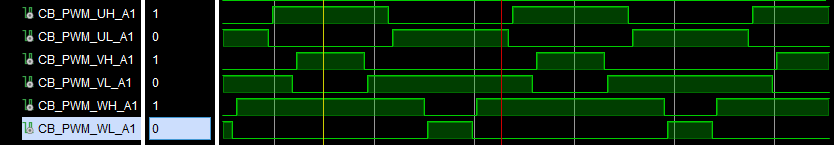
\includegraphics[width=0.80\textwidth, height=0.25\textwidth]{gfx/diagrams/PWM_Verification_with_diffferent_duty_cycle_waveforms.png}
	\caption{The \acs{PWM} Signals generated at the \acs{CB} with variable duty-cycle values}
	\label{fig:Implementation:PWM_Generated}
\end{figure}

\subsection{Block Design of \acs{PWM} Verification}
\label{sec:Implementation:Block_Design_PWM_verification}

The closed-loop \acs{PWM} verification architecture (refer figure \ref{fig:Implementation:CLOSED_LOOP_PWM_VERIFICATION}) is implemented to validate the functionality and accuracy of \acs{PWM} signals generated by the control board. In this configuration, control commands are transmitted to configure specific \acs{PWM} frequency and duty cycle values. The \acs{PS} of the \acs{MPSoC} parses these commands and communicates the relevant data to the \acs{CB} via \acs{UART}. The control board requires 2 bytes of data for the pwm\_f\_a1 command, which sets the \acs{PWM} frequency, and 5 bytes for the pwm\_d\_a1 command, which sets the duty cycle.

The control board generates six \acs{PWM} output signals, corresponding to three phases: Phase U High and Low, Phase V High and Low, and Phase W High and Low. These signals are interfaced directly with the \acs{FPGA}'s \acs{PL} section for real-time analysis.

\begin{figure}[t]
	\centering
	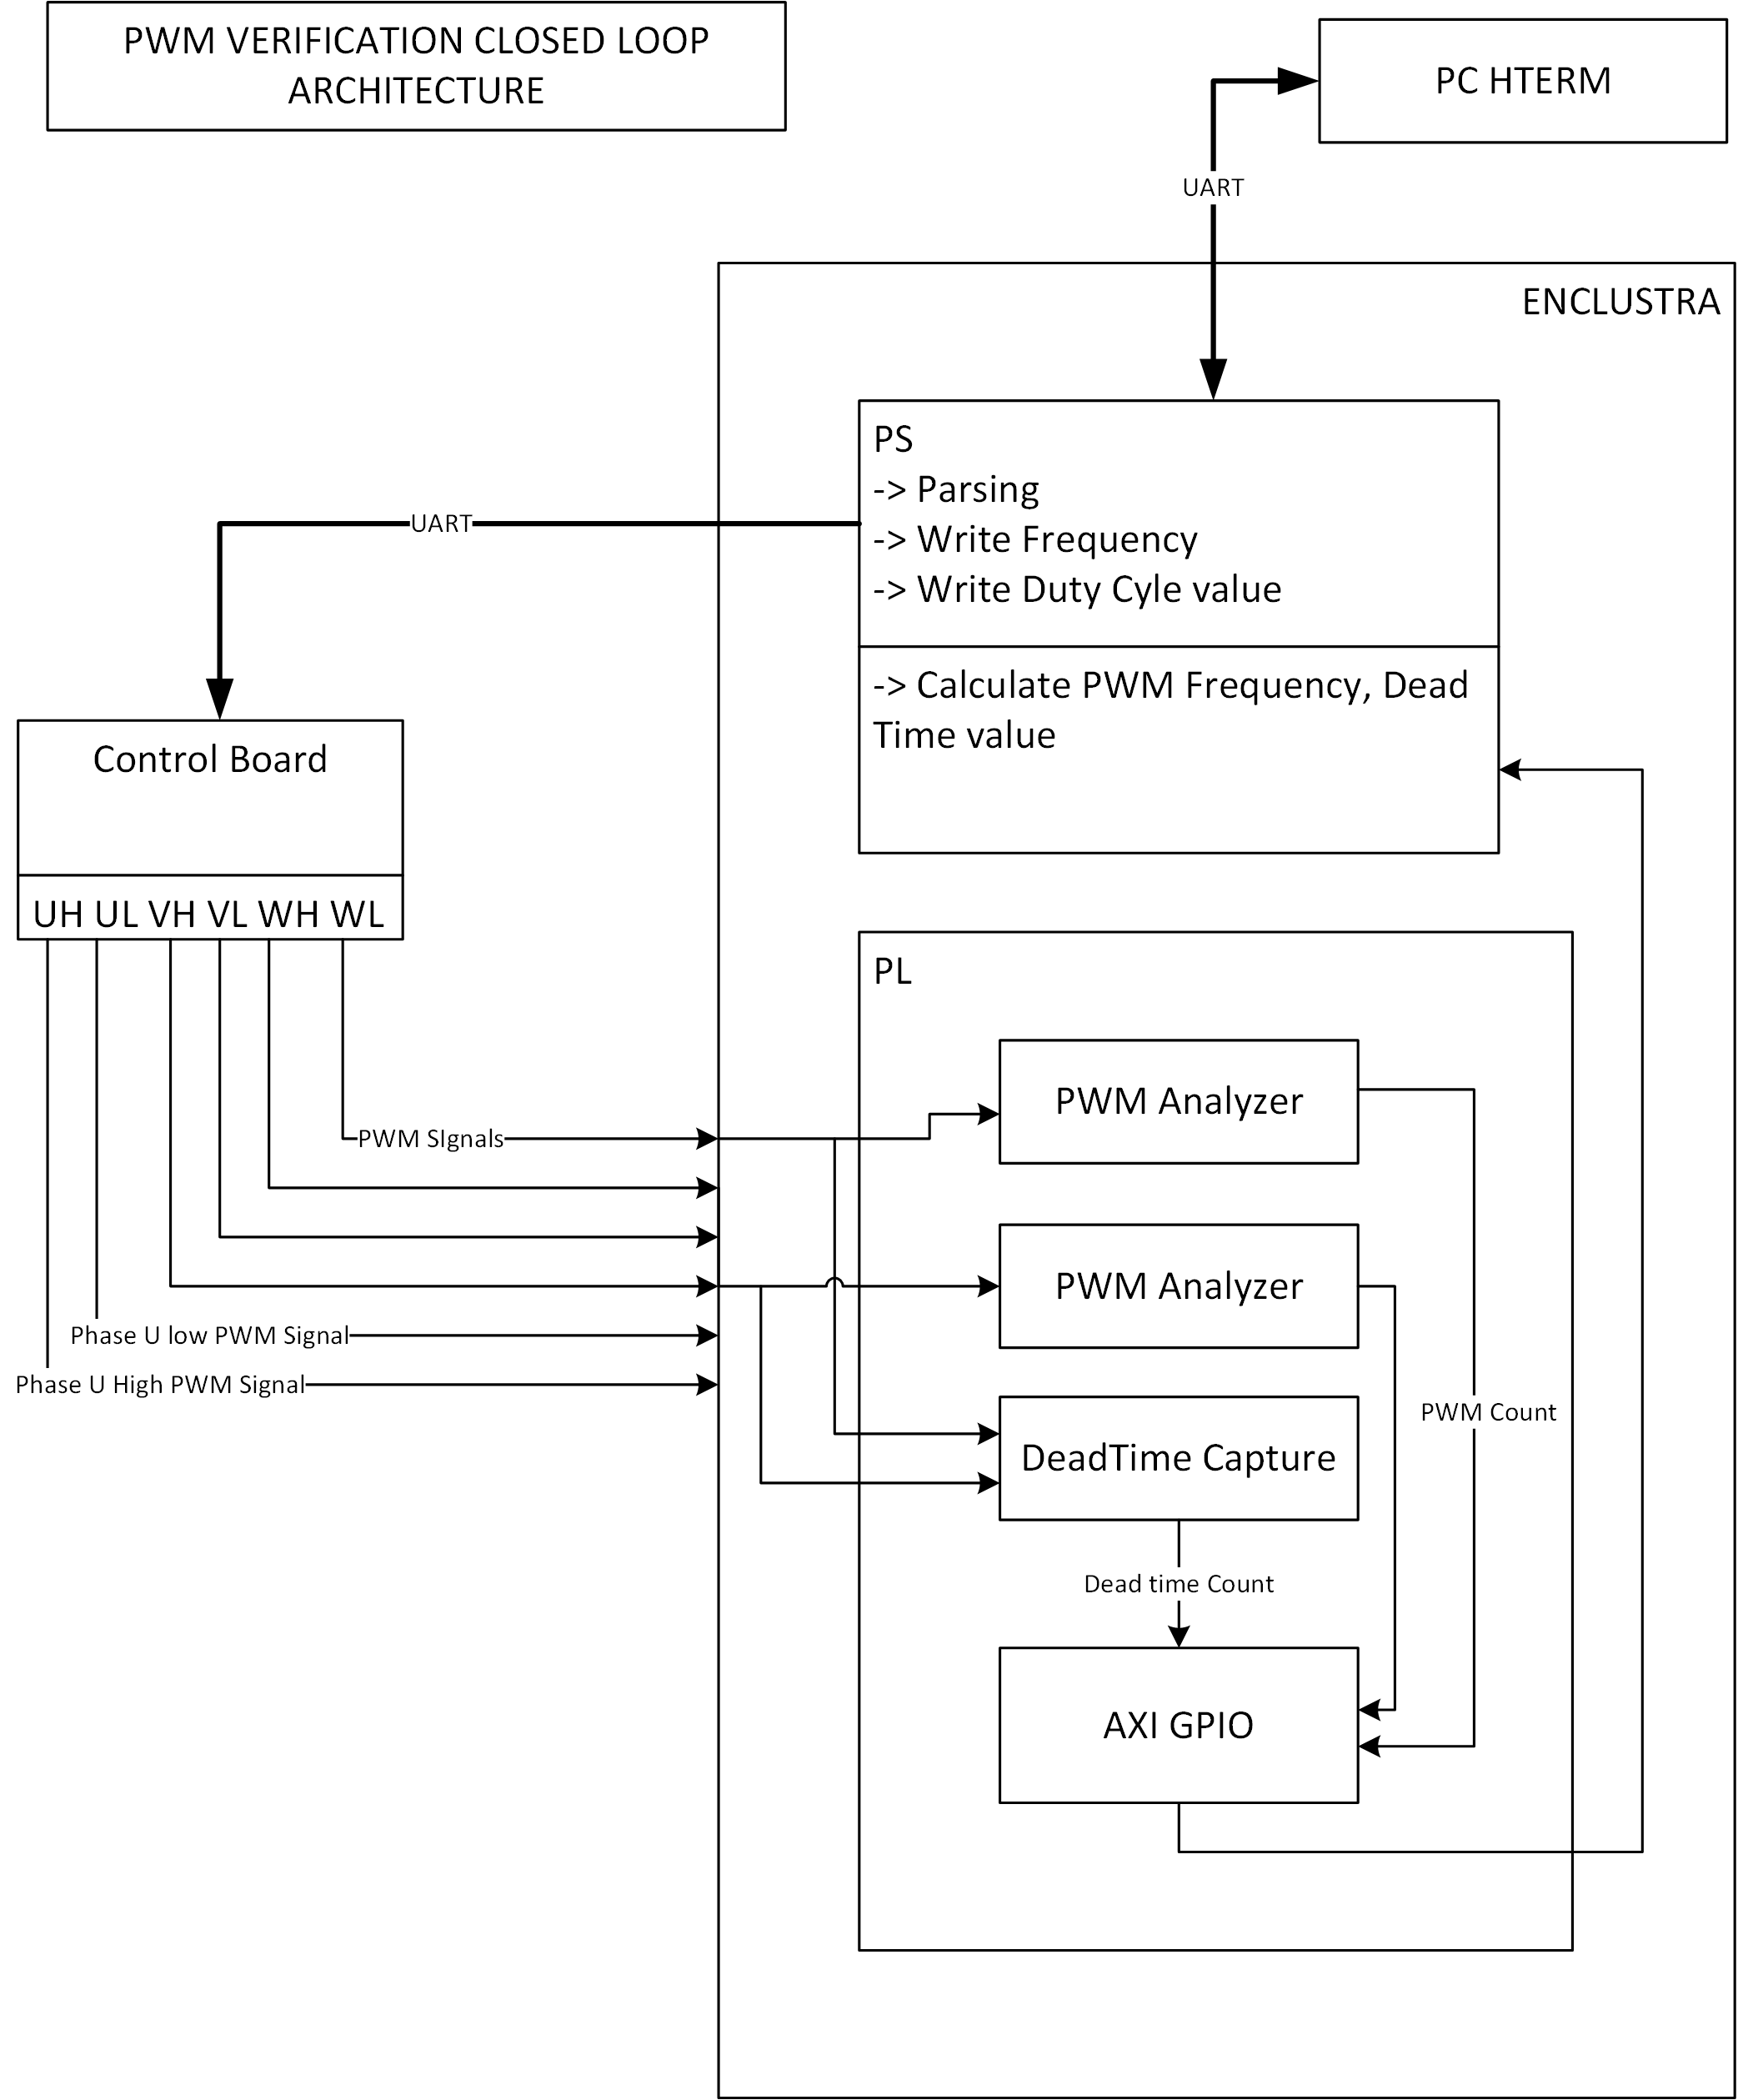
\includegraphics[width=0.60\textwidth]{gfx/diagrams/PWM_VErification.png}
	\caption{Block diagram depicting the closed-loop \acs{PWM} verification architecture, which demonstrates the interaction among the control board, SoM, and \acs{FPGA} based signal analysis modules}
	\label{fig:Implementation:CLOSED_LOOP_PWM_VERIFICATION}
\end{figure}

Within the \acs{PL}, \acs{PWM} Analyzer modules process the input \acs{PWM} signals and calculate both the total \acs{PWM} period and the effective duty cycle count in clock cycles for each phase. These values are communicated to the \acs{PS}, where further processing determines the actual \acs{PWM} frequency and duty cycle for each signal.

The DeadTime Capture module in the \acs{PL} monitors pairs of \acs{PWM} signals from the same phase (high and low) to determine dead time intervals. The captured dead-time counts are combined into a single 32-bit register that encodes the time intervals (clock cycles) between high-to-low and low-to-high transitions. This information is transmitted to the \acs{PS} via the \acs{PWM} Capture \acs{AXI} module to calculate the dead time for each phase.

This closed-loop verification approach enables precise monitoring of \acs{PWM} signal characteristics and inter-phase dead times, establishing a robust framework for validating the performance and timing integrity of the \acs{PWM} \acs{IP} block on the control board.

\subsection{\acs{PWM} Analyzer}
\label{sec:Implementation:PWM_Analyzer}

The \acs{PWM} Analyzer \acs{FPGA} subsystem measures the characteristics of an incoming \acs{PWM} signal, specifically its period and duty cycle, by counting high-speed system clock cycles between key signal transitions. The module identifies consecutive rising edges of the \acs{PWM} signal to determine the total period, while the number of clock cycles between the rising and falling edges is used to compute the duty-cycle duration. Both measurements are accumulated using 16-bit counters, as illustrated in Figure \ref{fig:Implementation:PWM_Analyzer}. In addition to these edge detectors, a free-running counter runs continuously while the system is active, enabling the logic to compute differences between edge timestamps. These calculated values are written to \acs{AXI}-accessible registers, from which the \acs{PS} can retrieve them. The \acs{PS} converts these clock-cycle counts into user-interpretable \acs{PWM} parameters such as frequency and duty cycle.          
                                                              
\begin{figure}[H]
\begin{center}
  \begin{tikzpicture}[>=Stealth, every node/.style={font=\small}]
	
	% Title
	%\node (title) {\small\textbf{PWM Analyzer}};
	
	% Rounded rectangle block with RTL text inside
	\node[draw, rounded corners=6pt, minimum width=3cm, minimum height=3cm] (pwmblock)
	{
		% Use a small minipage so line breaks inside node look tidy
		\begin{minipage}{5.6cm}\centering
			\textbf{RTL}
		\end{minipage}
	};
	
	% ===== INPUTS (left side, vertical stack) =====
	\node[anchor=east, left=1.0cm of pwmblock, yshift=8mm] (clk)   {clk};
	\node[anchor=east, left=1.0cm of pwmblock]                 (rstn)  {rst\_n};
	\node[anchor=east, left=1.0cm of pwmblock, yshift=-8mm]  (pwmin) {pwm\_in};
	
	% ===== OUTPUTS (right side, vertical stack) =====
	\node[anchor=west, right=1.0cm of pwmblock, yshift=4mm]  (pwmcount) {\acs{PWM}\_count[15:0]};
	\node[anchor=west, right=1.0cm of pwmblock, yshift=-4mm] (dutycount){dutycycle\_count[15:0]};
	
	% ===== STRAIGHT ARROWS INTO THE BLOCK (inputs) =====
	% We draw from the input node's east to the west edge of pwmblock at the same vertical level:
	\draw[->] (clk.east)   -- (pwmblock.west |- clk.east);
	\draw[->] (rstn.east)  -- (pwmblock.west |- rstn.east);
	\draw[->] (pwmin.east) -- (pwmblock.west |- pwmin.east);
	
	% ===== STRAIGHT ARROWS OUT OF THE BLOCK (outputs) =====
	\draw[->] (pwmblock.east |- pwmcount.west)  -- (pwmcount.west);
	\draw[->] (pwmblock.east |- dutycount.west) -- (dutycount.west);

  \end{tikzpicture}
\end{center}
\caption{\acs{PWM} Analyzer RTL Block Diagram}
\label{fig:Implementation:PWM_Analyzer}
\end{figure}

The verification platform operates at a 192 MHz system clock, whereas the \acs{PWM} signals under analysis arrive at significantly lower frequencies (16 kHz, 8 kHz, or 4 kHz) and originate from an independent clock domain. Direct sampling of these asynchronous signals introduces the risk of metastability, potentially leading to unpredictable behavior if input transitions violate flip-flop timing requirements. To ensure reliable operation, the incoming \acs{PWM} signal must be safely synchronized to the internal 192 MHz clock.

To address this issue, the \acs{PWM} Analyzer employs a three-stage flip-flop synchronizer, a well-established technique for transferring asynchronous signals into a synchronous clock domain. The synchronizer captures the incoming \acs{PWM} signal via three sequentially clocked registers, thereby significantly reducing the likelihood that metastability propagates into the measurement logic. A snippet of this synchronizer implementation is provided below. This approach ensures that subsequent period and duty-cycle measurements are performed on a clean, stable, and fully synchronized version of the \acs{PWM} waveform.

\begin{lstlisting}
	sync_pro : process(clk, rst_n)
	begin
		if rising_edge(clk) then
			if rst_n = '0' then
				PWM_sync_0 <= '0';
				PWM_sync_1 <= '0';
				PWM_sync   <= '0';
			else
				PWM_sync_0 <= PWM_in;
				PWM_sync_1 <= PWM_sync_0;
				PWM_sync   <= PWM_sync_1;
			end if;
		end if;
	end process sync_pro;
\end{lstlisting}

The \acs{PWM} signals originate from the control board, they are inherently asynchronous relative to the verification \acs{FPGA}’s internal clock domain. A further challenge occurs when the incoming \acs{PWM} signal becomes inactive for an extended period. Although the edge counters within the \acs{PWM} Analyzer stop incrementing when no additional transitions are detected, the previously stored count values remain unchanged. If the system reads these outdated values, the module may incorrectly indicate that a valid \acs{PWM} signal continues to exist. This behavior can result in misleading diagnostics or incorrect parameter estimations within the processing system.

A watchdog mechanism is integrated into the \acs{PWM} Analyzer architecture to address this issue. The watchdog detects extended inactivity on the synchronized \acs{PWM} input and ensures that all measurement counters are reset when the signal is absent. The watchdog logic includes an internal counter that increments whenever no \acs{PWM} edges, either rising or falling, are observed. While valid \acs{PWM} activity persists, this counter is periodically cleared. If the inactivity counter reaches a predefined threshold, the system interprets this as a loss of \acs{PWM} input. Upon exceeding this threshold, the watchdog resets the period and duty-cycle counters, thereby clearing any outdated measurement data. This approach ensures that the \acs{PWM} Analyzer does not retain obsolete timing values and provides an accurate indication of signal presence to the remainder of the system. The following code snippet illustrates a portion of the watchdog implementation.

\begin{lstlisting}
	watchdog_pro : process(clk,rst_n)       
	variable watchdog_counter : unsigned (16 downto 0) 
	:= (others => '0');        
	begin
		if rising_edge(clk) then
			if rst_n = '0' then
				watchdog_counter := (others => '0');
				watchdog_active <= '0';
			else
				if ((redge_pwm = '1') or (fedge_pwm = '1')) then
					watchdog_counter := (others => '0');
					watchdog_active <= '0';
				elsif watchdog_counter < WATCHDOG_LIMIT then
					watchdog_counter := watchdog_counter + 1;
					watchdog_active <= '0';
				else
					watchdog_counter := WATCHDOG_LIMIT;
					watchdog_active <= '1';
				end if;                
			end if;
		end if;
	end process watchdog_pro;
\end{lstlisting}

\subsection{Dead Time Capture}
\label{sec:Implementation:DeadTime}

Figure \ref{fig:Implementation:DeadTime_Capture} presents the architecture of the Dead Time Capture module implemented on the \acs{FPGA}. The module monitors complementary \acs{PWM} signals, specifically the high-side and low-side drive signals, and determines the dead time interval between their transitions. It detects the relevant signal edges on both inputs and measures the interval during which neither signal is active, a parameter critical to ensuring safe switching in power electronic systems.

The module stores the calculated dead time in a 32-bit output register, which the \acs{PS} accesses via the \acs{AXI} interface. This configuration enables the \acs{PS} to log, analyze, or process the timing data in a manner analogous to its handling of data from the \acs{PWM} Analyzer module.

\begin{figure}[htbp]
	\begin{center}
		\begin{tikzpicture}[>=Stealth, every node/.style={font=\small}]			
			% Title
			%\node (title) {\small\textbf{PWM Analyzer}};
			% Rounded rectangle block with RTL text inside
			\node[draw, rounded corners=6pt, minimum width=3cm, minimum height=3cm] (deadtimeblock)
			{
				% Use a small minipage so line breaks inside node look tidy
				\begin{minipage}{5.6cm}\centering
					\textbf{RTL}
				\end{minipage}
			};
			
			% ===== INPUTS (left side, vertical stack) =====
			\node[anchor=east, left=1.0cm of deadtimeblock, yshift= 8mm]   (clk)     {clk};
			\node[anchor=east, left=1.0cm of deadtimeblock, yshift= 4mm]   (rstn)    {rst\_n};
			\node[anchor=east, left=1.0cm of deadtimeblock, yshift= -4mm]  (pwmhigh) {pwm\_high};
			\node[anchor=east, left=1.0cm of deadtimeblock, yshift= -8mm]  (pwmlow)  {pwm\_low};
			
			% ===== OUTPUTS (right side, vertical stack) =====
			\node[anchor=west, right=1.0cm of deadtimeblock, yshift=0mm] (deadTime){deadTime\_count[31:0]};
			
			% ===== STRAIGHT ARROWS INTO THE BLOCK (inputs) =====
			% We draw from the input node's east to the west edge of pwmblock at the same vertical level:
			\draw[->] (clk.east)   -- (deadtimeblock.west |- clk.east);
			\draw[->] (rstn.east)  -- (deadtimeblock.west |- rstn.east);
			\draw[->] (pwmhigh.east) -- (deadtimeblock.west |- pwmhigh.east);
			\draw[->] (pwmlow.east) -- (deadtimeblock.west |- pwmlow.east);
			
			% ===== STRAIGHT ARROWS OUT OF THE BLOCK (outputs) =====
			\draw[->] (deadtimeblock.east |- deadTime.west)  -- (deadTime.west);			
		\end{tikzpicture}
	\end{center}
	\caption{Dead Time Capture RTL Block Diagram}
	\label{fig:Implementation:DeadTime_Capture}
\end{figure}

The Dead Time Capture module employs synchronization and signal-validation methods identical to those of the \acs{PWM} Analyzer block to ensure reliable operation. A three-stage flip-flop synchronizer safely transfers external \acs{PWM} signals into the \acs{FPGA} clock domain, while a watchdog unit continuously monitors signal activity. As in the \acs{PWM} Analyzer, the watchdog resets the internal dead time counters if no valid \acs{PWM} transitions occur within a specified interval, thereby preventing outdated or incorrect timing data from reaching the processing system.

The control board incorporates an \acs{OVC} protection module that detects overcurrent and short-circuit conditions. This module disables the \acs{PWM} outputs upon identification of a fault. Following the successful testing of the \acs{PWM} and CurrentSense pathways, the next objective is to verify the protection logic's functionality under fault scenarios. The following section details the \acs{OVC} verification process.

\section{\acs{OVC} Verification}
\label{sec:Implementation:OVC_Verification}

The \acs{OVC} module continuously monitors phase currents by capturing current-sense values generated by the \acs{SPI} module. These values are compared to configurable thresholds, which are adjustable via the \acs{PS} of the control board (RPU). Upon detection of an overcurrent or short-circuit condition (see Section \ref{sec:Conecpt:UnderstandingDUTs:OVC_Detect}), the \acs{OVC} module promptly disables the \acs{PWM} outputs to prevent equipment damage.

Figure \ref{fig:Implementation:OverCurrent_PWM_OFF_ControlBoard} presents the \acs{OVC} Protection module in conjunction with the \acs{PWM} OFF module as implemented on the control board. The \acs{PWM} OFF module functions as an error-signal detection system that tristates the \acs{PWM} output buffers when any of the following five error conditions are detected:

\begin{itemize}
	\item error\_1: ovc\_event from \acs{OVC} Detection (active-high and latched)
	\item error\_2: task\_overflow\_current\_control\_A from Scheduler (active-high)
	\item error\_3: watchdog\_error\_core0 from Scheduler (active-high)
	\item error\_4: watchdog\_error\_core1 from Scheduler (active-high)
	\item error\_5: GATE\_FLT\_Ax short-circuit from Power-Board (active-low)
\end{itemize}

\begin{figure}[t]
	\centering
	\includegraphics[width=0.80\textwidth,height=0.40\textheight]{gfx/diagrams/OverCurrent_PWM_OFF_Control_Board.png}
	\caption{Block diagram of the Overcurrent Protection \acs{FPGA} Implementation in the Control Board}
	\label{fig:Implementation:OverCurrent_PWM_OFF_ControlBoard}
\end{figure}

The default configuration parameters for the overcurrent protection system are as follows:

\begin{itemize}
	\item ovc\_offset = 0x800 $\approx$ 0A
	\item ovc\_low\_limit = 0x650 $\approx$ $\pm$ 65A (ovc\_event occurs)
	\item ovc\_timer = 0x280 $\approx$ 10 $\mu$s (running with 65MHz $\rightarrow$ waiting on ovc\_low\_limt before error indication)
	\item ovc\_high\_limit = 0x7CE $\approx$ $\pm$ 80.5A (ovc\_event occurs)
\end{itemize}

\subsection{Block Design of \acs{OVC} Verification}
\label{sec:Implementation:BlockDesign_OVC_Verification}

Verification of the \acs{OVC} protection module utilizes the setup shown in Figure \ref{fig:Implementation:OverCurrent_Verification_BD}. The testing methodology closely follows the procedure established for validating the Current Sense block, allowing for reuse of the \acs{DAC}-based signal generation and \acs{UART} communication interface with only minor modifications. In this test, a constant digital value is loaded into the \acs{DAC}, which is subsequently converted into an analog signal representing the measured phase current and applied to the control board.

If the simulated current exceeds the \acs{OVC} threshold of approximately ±65 A, the protection logic activates the overcurrent indicator for the corresponding phase. The system monitors the duration for which the signal remains above this threshold. Should the overcurrent condition persist beyond the 10 μs internal timeout, the module identifies it as a genuine fault and asserts the ovc\_event output. The design also provides rapid protection against severe faults: if the sensed value exceeds the upper ±80.5 A boundary, the module immediately classifies the event as a short-circuit condition. In this scenario, the short-circuit flag is set immediately, and ovc\_event is triggered without delay.

In addition to transmitting the \acs{OVC}\_Verification control commands (ovc\_u\_a1, ovc\_v\_a1, ovc\_w\_a1), the \acs{FSM} in the Verification \acs{MPSoC} writes to the \acs{DAC}. The \acs{OVC} module on the control board then captures the following signals and transmits them via \acs{UART} back to \acs{MPSoC} for further processing in the \acs{PS}, using a two-byte format:

\begin{itemize}
	\item Byte 0: ovc\_status[0:5] (active high) \newline
	$\rightarrow$  Bit 0 – overcurrent on phase U \newline
	$\rightarrow$  Bit 1 – short circuit on phase U \newline
	$\rightarrow$  Bit 2 – overcurrent on phase V  \newline
	$\rightarrow$  Bit 3 – short circuit on phase V \newline
	$\rightarrow$  Bit 4 – overcurrent on phase W  \newline
	$\rightarrow$  Bit 5 – short circuit on phase W \newline
	\item Byte 1: Bit 0 - ovc\_event - overcurrent error indication (active high) 
\end{itemize}

\begin{figure}[H]
	\centering
	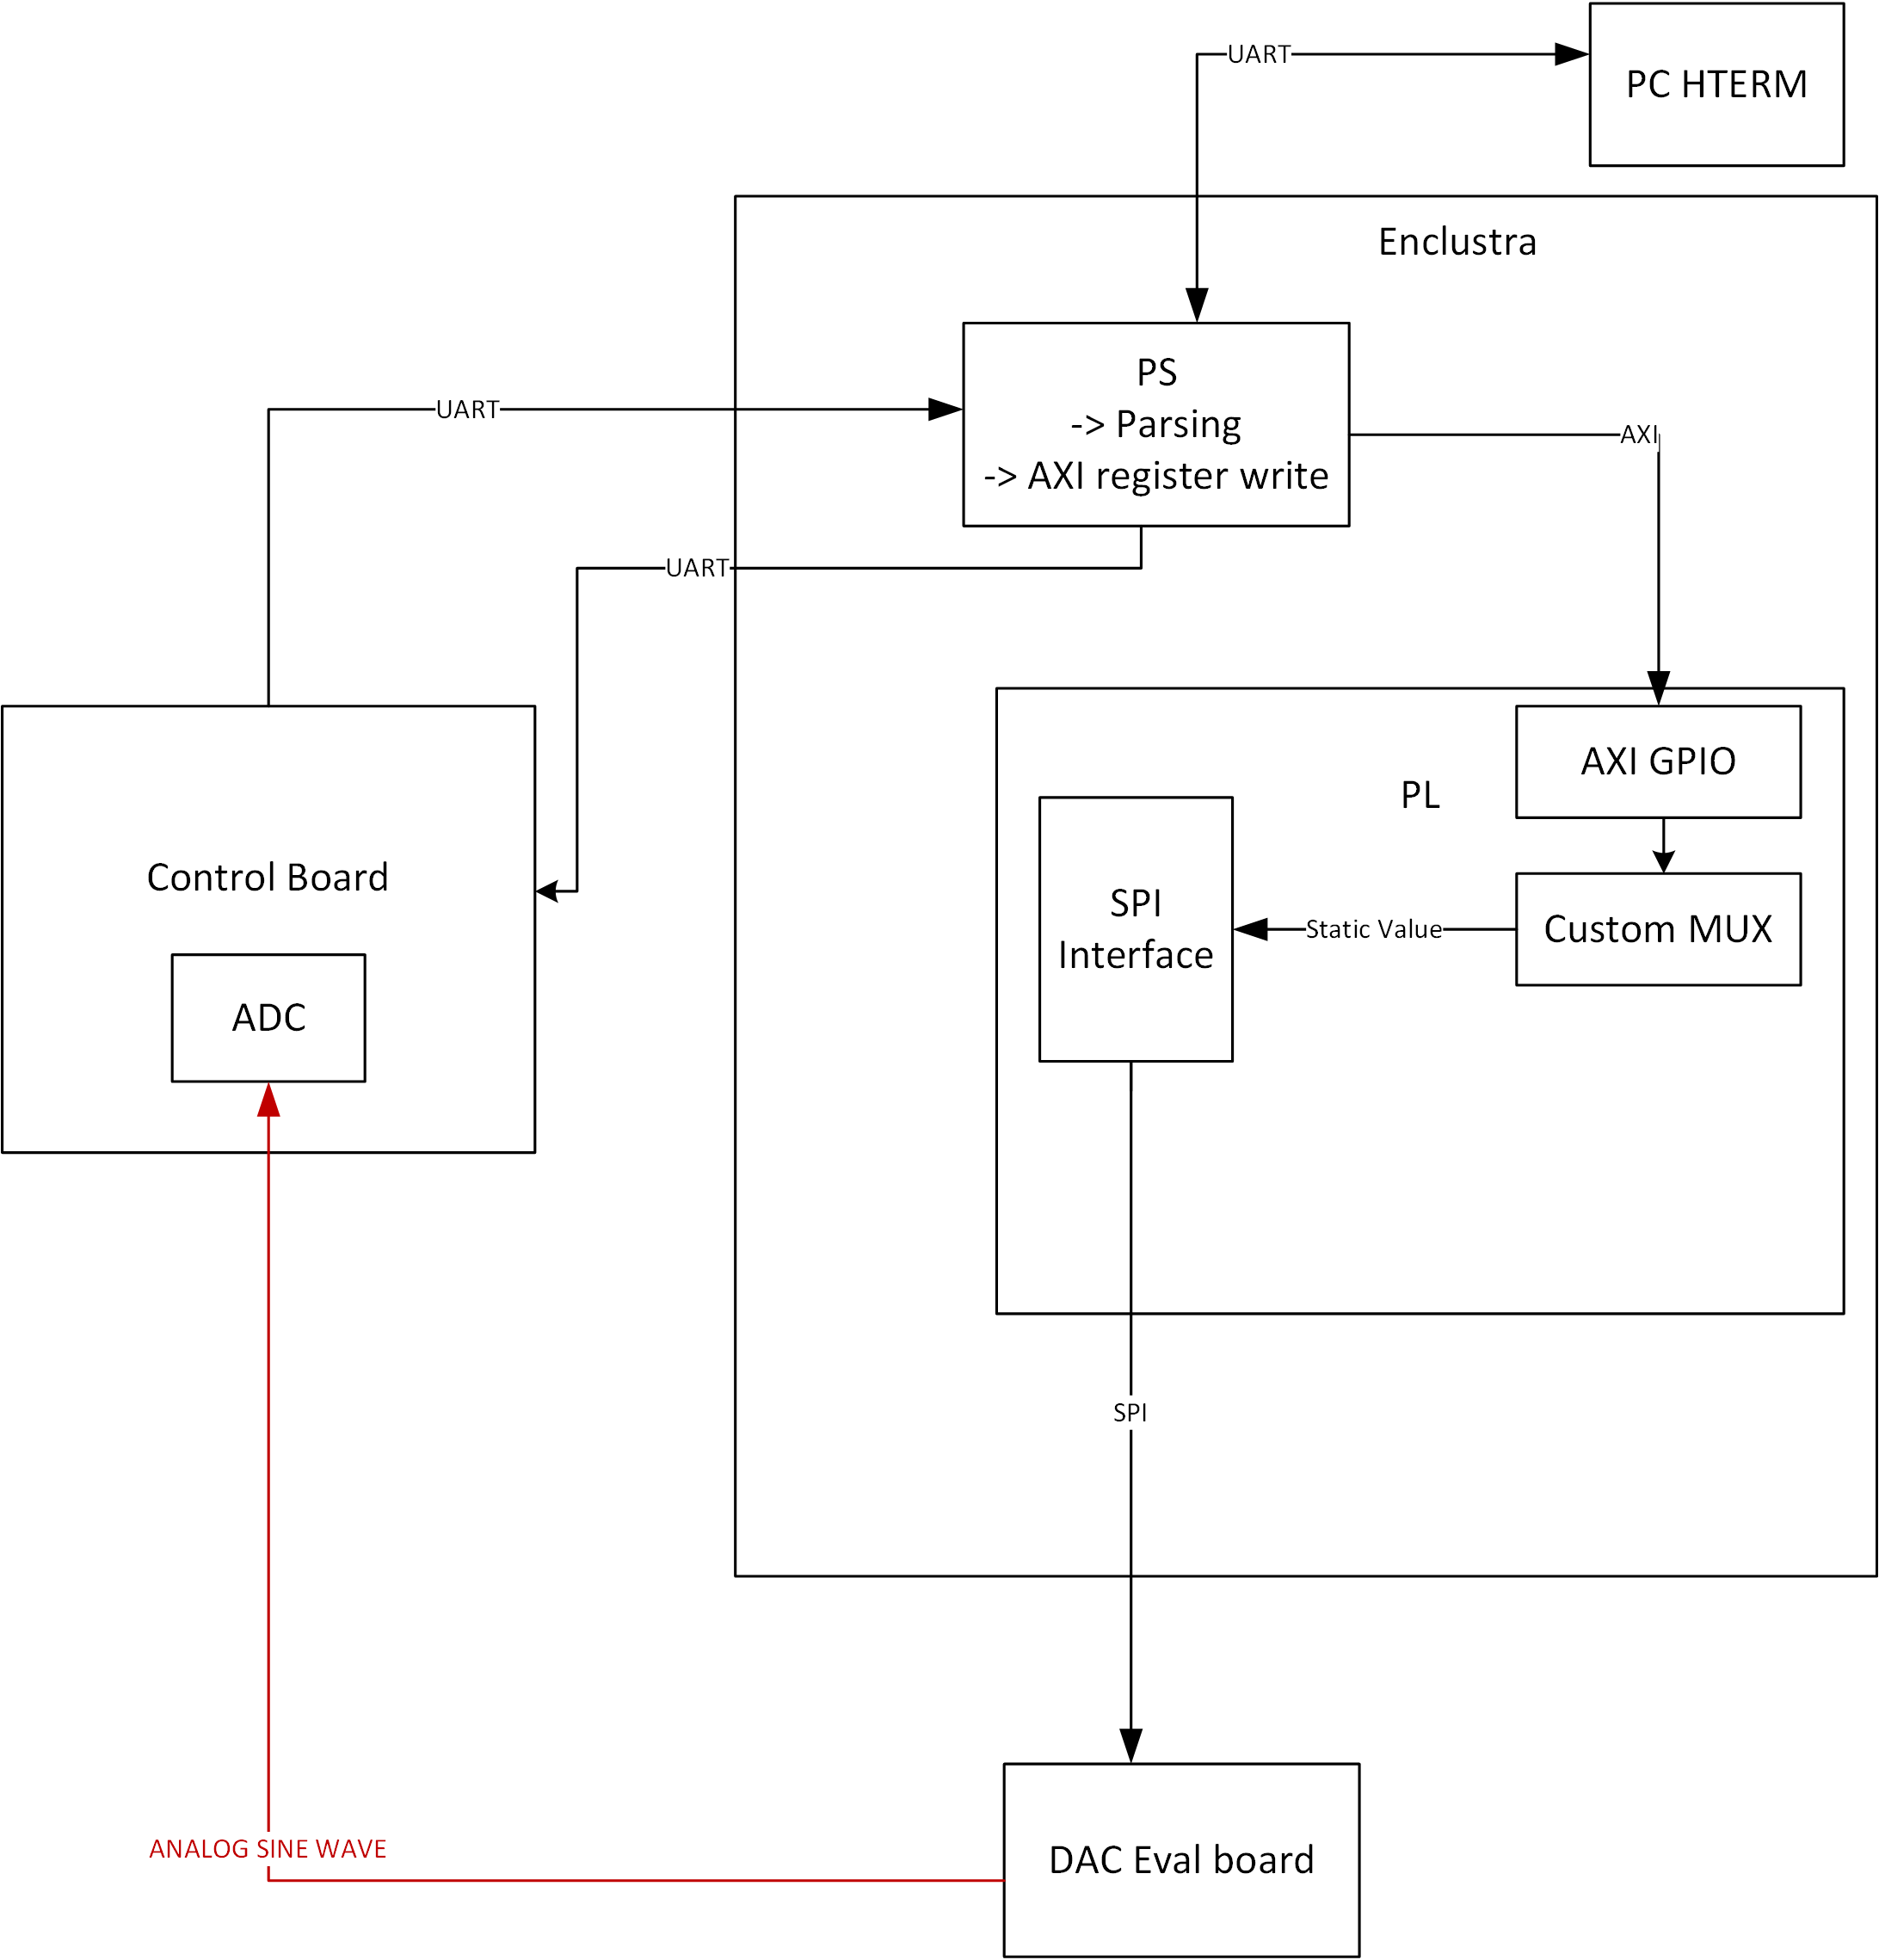
\includegraphics[width=0.70\textwidth]{gfx/diagrams/OVC_Verification.png}
	\caption{Block Design of the Overcurrent Verification setup: Note that apart from the \acs{DDFS}, the same analog path is reused for \acs{OVC} Verification}
	\label{fig:Implementation:OverCurrent_Verification_BD}
\end{figure}
 
Previous sections have examined the functional blocks within the \acs{PL} and the hardware mechanisms responsible for signal generation, measurement, and real-time control. The following section addresses the \acs{PS}, which executes software to supervise and coordinate these hardware modules. Within the \acs{PS}, a dedicated Verification Controller finite state machine manages user interaction via \acs{UART}, facilitates communication with \acs{PL} blocks, and validates feedback from the \acs{PL} modules. The \acs{PS} is also responsible for higher-level tasks such as \acs{FFT} processing, frequency estimation, and duty-cycle calculation, which constitute the core of the verification framework. This co-design of software and hardware results in a tightly integrated system, enabling complex processing tasks to operate alongside deterministic logic operations to ensure accurate and reliable system behavior.
  
\section{Processing Subsystem application}
\label{sec:Implementation:PS_Application}

The servo drive control board \acs{FPGA} verification application utilizes one of the A53 processor cores from the \acs{MPSoC}. The verification controller \acs{FSM} (see figure \ref{fig:Implementation:verificationontroller_fsm}) manages both user interaction and validation of feedback from the \acs{PL}, serving as the backbone of the verification platform.

\subsection{Communication and Data Handling Layer}
\label{sec:Implementation:Communication_and_DataHandling}

The Processing Subsystem employs two distinct \acs{UART} interfaces (refer figure \ref{fig:concept:PoC}) on the Zynq UltraScale+ \acs{MPSoC} to facilitate communication with external devices and \acs{PL}. UART0 establishes a connection with the host PC for command transmission, runtime configuration, and reporting of verification results. UART1 serves as a data exchange interface between the verification \acs{MPSoC} and the servo control board, managing measurement data, trigger signals, and diagnostic responses during validation.

Distinct communication strategies are implemented for each interface to maintain reliability under varying data rates and unpredictable traffic conditions. UART0 utilizes interrupt-driven reception and transmission. Interrupts are triggered by the arrival of new data, timeouts, or the emptying of the transmit \acs{FIFO}. The interrupt handler processes incoming data, and promptly prepares the \acs{UART} driver for subsequent messages. This configuration enables non-blocking interaction with the PC terminal, allowing the Verification Controller's \acs{FSM} to operate independently of user input delays.

UART1 similarly employs interrupt handling, however, all incoming bytes are stored in a software ring buffer to prevent data loss during burst transfers. The UART1 interrupt service routine copies new data into the circular buffer for later parsing. This method separates rapid data collection from slower processing tasks, ensuring that no data is lost between verification calls.

During system initialization, both \acs{UART} modules are configured by setting up the XUartPs drivers, specifying the baud rates (115200 Bd for the PC and 921600 Bd for the control board), and registering interrupt handlers with the Generic Interrupt Controller (GIC). Interrupts are configured to trigger on receive-full, timeout, and overrun events, ensuring that the firmware remains informed of critical communication events.

These interfaces collectively serve as the primary communication link for the verification platform, enabling data exchange, and efficient coordination \acs{PS}, \acs{PL}, and external control hardware.

\subsection{Verification Controller fsm}
\label{sec:Implementation:Verification_Controller_fsm}

Control commands are transmitted from the user to the system via UART0. These commands specify the verification procedure to be executed. A command parser within the \acs{PS} interprets each incoming command and initiates the appropriate verification routine. The supported control commands are summarized below:

As shown in Table \ref{table:Control_Commands_Verification}, when the \acs{FSM} receives a control command, it splits the command string at each underscore. If the initial segment corresponds to a motor phase, such as "phu," "phv," or "phw," the \acs{FSM} transitions to the CurrentSense\_Verification state. In this state, the \acs{AXI} register for the selected phase is updated according to the command. The \acs{FSM} then examines the subsequent segment of the command. If it identifies "s," the \acs{FSM} transitions to the CurrentSense\_Static state. If it identifies "d," it transitions to the CurrentSense\_Dynamic state. In the CurrentSense\_Static state, a predetermined static value is transmitted to the \acs{DAC} to generate a constant analog signal. The system can perform either a single static test or a sequence of tests. For multiple tests, a series of 16-bit values ranging from 0x0000 to 0xFFFF is written to the \acs{DAC} to simulate various analog conditions. The \acs{DAC} output is connected to the control board's \acs{ADC}. The control board responds to these static analog inputs by providing 12-bit feedback to the verification \acs{MPSoC} via UART1 (refer to section \ref{sec:Implementation:Current_Sense_Verification}).

\begin{table}[H]
	\centering
	\caption{\textbf{Overview of Control Commands and Corresponding Verification Functions}}
	\label{table:Control_Commands_Verification}
	\setlength{\fboxsep}{0pt} % box padding
	\renewcommand{\arraystretch}{1.2} % increase row height for spacing
	\fbox{%
		\begin{tabularx}{\textwidth}{|>{\raggedright\arraybackslash}p{4cm}|>{\raggedright\arraybackslash}p{4cm}|>{\raggedright\arraybackslash}X|}
			\hline
			\textbf{Control Command(s)} & \textbf{Verification Type} & \textbf{Description} \\
			\hline
			\verb|phu_s_a1|, \verb|phv_s_a1|, \verb|phw_s_a1| & Current Sense Static Verification &
			Instruct the verification controller fsm to perform static current-sense validation for phases U,V and W respectively\\ 
			\hline
			\verb|phu_d_a1|, \verb|phv_d_a1|, \verb|phw_d_a1| & Current Sense Dynamic Verification &
			Performs dynamic current-sense verification for the specified phase. \\ 
			\hline
			\verb|pwm_v| & PWM Module Verification &
			Triggers the PWM verification sequence. Internally the \acs{FSM} sends \verb|pwm_f_a1| together with the desired frequency value to configure the PWM frequency, and \verb|pwm_d_a1| with the corresponding duty-cycle value to adjust the PWM duty cycle. \\ 
			\hline
			\verb|ovc_u_a1|, \verb|ovc_v_a1|, \verb|ovc_w_a1| & \acs{OVC} Module Verification &
			Triggers over-current (\acs{OVC}) verification for the requested phase.\\ 
			\hline
		\end{tabularx}%
	}
\end{table}

\begin{figure}[H]
	\centering
	\includegraphics[width=1.00\textwidth, height=1.00\textheight]{gfx/diagrams/Processing_Subsystem_Statemachine.png}
	\caption{Verification Controller \acs{FSM}}
	\label{fig:Implementation:verificationontroller_fsm}
\end{figure}

\subsection{Signal Acquisition and Spectral Analysis}
\label{sec:Implementation:signal_Acquistion}

Upon detection of the command token "d," the \acs{FSM} (figure \ref{fig:Implementation:verificationontroller_fsm}) transitions to the CurrentSense\_Dynamic state. In this state, a trigger signal instructs the \acs{FPGA} \acs{PL} modules to initiate the \acs{DDFS} module, which generates a 1 kHz sine wave for dynamic verification. Following activation of the \acs{DDFS} module, the \acs{PS} awaits the receipt of 4096 samples from the control board. These samples are transmitted over UART1 in 8-bit segments and stored in a ring buffer within the \acs{PS} for subsequent processing.

The control board transmits 12-bit \acs{ADC} values, whereas the \acs{FPGA} \acs{DDFS} module generates 16-bit digital samples. For comparison, the raw data received via \acs{UART} must be reconstructed and appropriately scaled. Initially, two 8-bit bytes are combined to form a single 16-bit word using the following expression:

%\begin{align*}
%	\text{dynamic\_data\_buffer[i]} = (\text{(uint16\_t)}\, \text{data1} \ll \text{8}) \, | \, \text{data2} 
%\end{align*}

\begin{lstlisting}
dynamic_data_buffer[i] = ((uint16_t)data1 << 8) | data2;
\end{lstlisting}

In this process, the first byte (data1) is shifted left by 8 bits to occupy the higher portion of the word, and the second byte (data2) is combined using a bitwise OR operation. This method reconstructs the original sample transmitted over \acs{UART}.

Subsequently, the 12-bit \acs{ADC} values are converted to analog voltage levels, providing a consistent reference for comparison with the \acs{DDFS} module's 3.3 V output. The conversion is performed using the following formula:

\begin{lstlisting}
decData = ((float32_t)hwData / pow(2, 12)) * 3.3;
\end{lstlisting}

In this context, hwData represents the raw 12-bit \acs{ADC} reading. Dividing by $2^{12}$ normalizes the value to a fraction of the full scale, and multiplying by 3.3 V converts it to the actual voltage at the \acs{DAC} output. Expressing both the control board and \acs{FPGA} reference signals in voltage units facilitates direct comparison, despite differences in bit resolution.

The voltage data is subsequently processed using a \acs{FFT} to analyze its frequency content. The resulting spectral peak is compared to the expected 1 kHz sine wave generated by the \acs{DDFS} module. This comparison verifies the accuracy of the control board’s dynamic current-sense response. Utilizing voltage units also mitigates errors arising from differences in bit resolution, thereby enhancing the reliability and precision of the verification process.

After reconstructing and converting dynamic current-sense samples to voltage values, the system verifies that the control board generates the expected 1 kHz sinusoidal waveform via spectral analysis. This process is managed by two primary functions: \textbf{fft\_func()}, which computes the frequency spectrum, and \textbf{dynamicTestError\_calculations()}, which compares the measured waveform to the reference based on frequency, amplitude, and RMS values.

To enable accurate and efficient analysis on the ARM Cortex-A53 core, the system utilizes the \acs{CMSIS-DSP} library, a signal-processing framework developed by ARM. \acs{CMSIS-DSP} provides optimized routines for fast FFTs, statistical analysis, vector mathematics, and filtering. The \acs{FFT} function implemented, \textbf{arm\_rfft\_fast\_f32()}, employs pre-computed twiddle factors and radix-based algorithms specifically designed for ARM processors. This configuration reduces computational overhead and supports real-time verification, even with large sample sizes such as 4096 points. Using \acs{CMSIS-DSP} enables the system to achieve predictable timing, reliable numerical accuracy, and reduced CPU usage compared to a manual \acs{FFT} implementation.

\begin{enumerate}
	\item \underline{\textbf{\acs{FFT} Computation (fft\_func())}}
	
	The fft\_func() function identifies the primary frequency component in the signal and verifies whether the measured waveform corresponds to the expected 1 kHz output from the \acs{DDFS} module. 
	
	\begin{lstlisting}
arm_rfft_fast_init_f32(&S, FFT_SIZE);
arm_mean_f32(dynamic_data_decimal_buffer, FFT_SIZE, &mean);
	\end{lstlisting}

	The \acs{FFT} is configured to use 2048 points. Initially, the mean value of the input buffer is calculated and subtracted from each sample. Removal of the \acs{DC} offset is essential for several reasons:
	
	\begin{itemize}
		\item It prevents the \acs{DC} component from dominating the frequency spectrum.
		\item It reduces spectral leakage within the frequency analysis.
		\item It ensures accurate identification of the true dominant frequency component.
	\end{itemize}
	
	\textbf{\acs{FFT} Execution}
	
	The CMSIS function executes a real \acs{FFT} directly on the input data.
\begin{lstlisting}
arm_rfft_fast_f32(&S, dynamic_data_decimal_buffer, 
fft_output_buffer, 0);
\end{lstlisting}
	The output is a set of interleaved real and imaginary values, requiring magnitude computation for each \acs{FFT} bin.
	
	\textbf{Magnitude Extraction}
	
	The magnitude of each frequency component can be determined using the following formula:
	
	\begin{align*}
		\text{mag}[k] &= \sqrt{(Re\{X[k]\})^{2} + (Im\{X[k]\})^{2}}
	\end{align*}
	
	This calculation should be repeated for each bin up to the Nyquist frequency:
	
\begin{lstlisting}
for (int i = 1; i < (FFT_SIZE / 2); i++) {
	float32_t real = fft_output_buffer[2 * i];
	float32_t imag = fft_output_buffer[2 * i + 1];
	magnitude_buffer[i] = sqrtf(real * real + imag * imag);
}
\end{lstlisting}

	\textbf{Peak Frequency Identification}
	
	CMSIS provides a function to efficiently identify the bin with the highest magnitude:
	
\begin{lstlisting}
arm_max_f32(magnitude_buffer, (FFT_SIZE/2) + 1, 
&max_val, &max_index);
\end{lstlisting}
	Each bin corresponds to a frequency, which is calculated as follows:
	
	\begin{align*}
		\text{bin width} &= \frac{F_s}{N}
	\end{align*}
	where $F_s$ (Sampling frequency of the Control Board \acs{ADC}) = 984,615.3846 Hz. The measured frequency can then be determined as follows:
	
\begin{lstlisting}
freq = max_index * bin_width;
\end{lstlisting}
	This calculation yields the primary sinusoidal frequency present in the received signal.
	
	\item {\underline{\textbf{Dynamic Error Calculation (dynamicTestError\_calculations())}}}
	
	The function determines the fidelity of the measured signal in comparison to the ideal reference sinusoid produced by the \acs{DDFS} module.
	
	\textbf{Frequency Error}
\vspace{0.5\baselineskip}
\begin{lstlisting}
error_f = 100/REF_MAX_FREQUENCY * 
fabsf(REF_MAX_FREQUENCY - freq);
\end{lstlisting}

	This expression quantifies the percentage deviation of the measured frequency from the expected value of 1 kHz. 
	
	\textbf{Amplitude Error}
	
	Amplitude is determined by measuring the peak-to-peak value of the buffered signal. This step also identifies gain-related errors within the control board’s sensing path.

\begin{lstlisting}
error_amp = 100/REF_PEAK2PEAK_VALUE * 
(REF_PEAK2PEAK_VALUE - 
peak2peak_f32(dynamic_data_decimal_buffer_copy, FFT_SIZE));
\end{lstlisting}

	\textbf{RMS Error}
	
	The root mean square (RMS) value is calculated using the CMSIS library. 
	
\begin{lstlisting}
arm_rms_f32(dynamic_data_decimal_buffer_copy, 
FFT_SIZE, &rms_result);
\end{lstlisting}

	The RMS error is significant because it reflects both the amplitude and the waveform shape.

\begin{lstlisting}
error_rms = 100/REF_RMS_VALUE * (REF_RMS_VALUE - rms_result);
\end{lstlisting}

	\textbf{Pass/Fail Evaluation}

The system accepts the measurement if all three errors remain below 5%.

\begin{lstlisting}
if ((error_f<5.0f) && (error_amp<5.0f) && (error_rms<5.0f))
dynamicTestResult_passed();
else
dynamicTestResult_failed();
\end{lstlisting}
\end{enumerate}

The two functions described above are essential to the dynamic verification process. The fft\_func() function uses a CMSIS-optimized real \acs{FFT} to analyze the spectrum and identify the main frequency in the reconstructed voltage samples. The dynamicTestError\_calculations() function evaluates frequency deviation, amplitude accuracy, and RMS values against reference points. Together, these functions verify that the control board’s dynamic current-sense path accurately reproduces the 1 kHz sinusoidal test signal from the \acs{DDFS} module. \acs{CMSIS-DSP} ensures strong performance, reliable calculations, and consistent signal processing, which are critical for comprehensive \acs{MPSoC}-based hardware testing.

\subsection{Pulse-based Signal Evaluation}
\label{sec:Implementation:Pulse_Based_Signal_Evaluation}

When the command parser detects the token "pwm", the fsm transitions from the Parse\_command state to the \acs{PWM}\_Verification state (see figure \ref{fig:Implementation:verificationontroller_fsm}). This process verifies the \acs{PWM}\_IP (\acs{FPGA}) module's ability  to generate the \acs{PWM} signals with specified frequencies and duty cycles. As outlined in the state-machine diagram (figure \ref{fig:Implementation:verificationontroller_fsm}), the \acs{PWM} verification routine employs an automated procedure in which the \acs{PS} sets three distinct \acs{PWM} carrier frequencies: 16 kHz, 8 kHz, and 4 kHz. For each frequency, three specific duty-cycle settings are tested, yielding a total of 9 \acs{PWM} scenarios. Each scenario is recorded and evaluated by the Verification \acs{MPSoC}.
 
The \acs{PWM} module on the control board generates six outputs corresponding to the high-side and low-side switching signals for each of the three motor phases.

\begin{itemize}
	\item Phase U: UH (high-side), UL (low-side)
	\item Phase V: VH (high-side), VL (low-side)
	\item Phase W: WH (high-side), WL (low-side)
\end{itemize}

During each test, all six signals operate at the same switching frequency, while their duty cycles vary according to patterns defined by the Processing Subsystem. The \acs{PWM}\_IP Verification is initiated by the \acs{PS} through the sequential transmission of four \acs{UART} commands:

\begin{enumerate}
	\item The first command, pwm\_f\_a1, indicates that the subsequent payload will specify the pwm frequency.
	\item The second command transmits the encoded 16-bit frequency value, such as 16000 Hz, 8000 Hz, or 4000 Hz. 
	\item After the frequency is confirmed, the \acs{FSM} transitions to the \acs{PWM}\_setDutyCycle state. The third command, pwm\_d\_a1, then indicates that the subsequent payload specifies the duty-cycle settings.
	\item The fourth command transmits the the duty-cycle settings as a 40-bit value, which includes three duty-cycle values for the high-side switches of phases U, V, and W. The system selects the appropriate duty-cycle pattern from predefined tables, such as duty\_16k[], duty\_8k[], or duty\_4k[], according to the current frequency. After transmitting the duty-cycle values, the system introduces a brief delay using usleep to allow the control board’s \acs{PWM} generator to adjust before recording the results.
\end{enumerate}

In the \acs{PWM}\_Capture state (figure \ref{fig:Implementation:verificationontroller_fsm}), the \acs{PS} retrieves \acs{PWM} measurement results from the \acs{FPGA}’s \acs{AXI}-based \acs{PWM} capture \acs{IP} block. This custom module records the following parameters:

\begin{itemize}
	\item \textbf{The \acs{PWM} period count} (from which the switching frequency is derived),
	\item \textbf{The ON-time count} (used to calculate the duty cycle),
	\item \textbf{The dead-time counter values} for both High→Low (HL) and Low→High (LH) transitions.
\end{itemize}

The \acs{PS} obtains these measurements by accessing specific memory-mapped \acs{AXI} register offsets corresponding to each phase and switching leg. For example:

\begin{itemize}
	\item \textbf{PHASE\_UH\_FREQUENCY\_DUTYCYCLE} returns a 32-bit word encoding the UH period and duty values.
	\item \textbf{PHASE\_U\_DEADTIME} provides the dead-time timestamps for phase U.
\end{itemize}

The \acs{PS} application decodes these raw register values. The lower 16 bits represent the \acs{PWM} period ($T_{PWM}$), while the upper 16 bits contain the duty-cycle count ($T_{ON}$). The \acs{PWM} frequency and duty cycle are calculated as follows:

\begin{align*}
	f_{PWM} &= \frac{192 MHz}{T_{PWM}}, \qquad Duty(\%) = \frac{T_{ON}}{T_{PWM}} \times 100
\end{align*}

The 192 MHz frequency reference corresponds to the clock that drives the PWM capture logic. This reference enables accurate conversion of clock counts to real signal characteristics.

Dead-time values are also converted to microseconds:

\begin{align*}
	Deadtime[\mu s] &= \frac{DT\_count}{192 MHz} \times 10^6
\end{align*}

This conversion ensures that the dead-time behavior of the control board’s gate-drive logic is measured accurately and can be compared across test runs. After decoding measurements for all six outputs (UH, UL, VH, VL, WH, WL), the \acs{PS} generates a structured text report. This report is transmitted over \acs{UART} and includes the following information:

\begin{itemize}
	\item \acs{PWM} frequency of each phase’s high-side and low-side switch,
	\item Duty cycle accuracy,
	\item High→Low and Low→High dead-time durations.
\end{itemize}

The \acs{FSM} increments the duty-cycle index. After completing all three duty-cycle patterns for the current frequency, the system advances to the next frequency. Upon completion of all nine scenarios (three frequencies and three duty cycles), the \acs{FSM} returns to the Idle state and awaits the next user command.

This automated verification process ensures that the control board’s \acs{PWM}\_IP \acs{FPGA} module meets the stringent timing requirements of motor-control applications. By evaluating all switching legs (UH/UL, VH/VL, WH/WL), the system verifies Frequency stability across all phases, Duty-cycle accuracy and linearity, Dead-time symmetry and correctness, Compliance with expected motor-control pulse patterns. The Verification MPSoC hardware directly captures the \acs{PWM} signals, and the \acs{PS} software decodes them. This configuration provides independent, high-resolution measurements of \acs{PWM} behavior. 

\subsection{Protection Event Monitoring}
\label{sec:Implementation:ProtectionEventMonitoring}

The \acs{OVC} Protection module verification ensures that the Control Board \acs{MPSoC} correctly detects and reports the over-current events under test conditions. The verification procedure shares conceptual similarities with the static path used in the Current Sense module. A single static value is transmitted to the \acs{DAC} path of the Verification \acs{MPSoC}, activating the \acs{OVC} \acs{FPGA} module on the Control Board. In contrast to current measurement tests, the \acs{OVC} module provides only event and status information rather than data samples.

Upon detection of the "ovc" token by the command parser, the Processing Subsystem \acs{FSM} transitions from the Parse\_command state to the \acs{OVC}\_Verification state (refer to the verification controller state machine diagram \ref{fig:Implementation:verificationontroller_fsm}) . Within this state, the Verification \acs{MPSoC} writes a user-defined synthetic current value  to the \acs{DAC} and Subsequently, the \acs{OVC} status and event codes are returned from the control board to the Verification \acs{MPSoC} via UART1, enabling comprehensive validation of the hardware module.

When the \acs{FSM} enters the \acs{OVC}\_Verification state, the \acs{PS} requests a 16-bit hexadecimal current value from the user. o ensure input validity, the buffer is examined using a dedicated function:

\begin{lstlisting}
bool is_valid_16bit_hex(const char *str);
\end{lstlisting}

This function verifies the following conditions:
\begin{itemize}
	\item The input adheres to the format 0xNNNN.
	\item Only valid hexadecimal characters are present.
	\item If the input is invalid, the \acs{PS} instructs the user to restart the test.
\end{itemize}

Following validation, the hexadecimal string is converted to a 16-bit integer using the following method:

\begin{lstlisting}
hexValue = (uint16_t)strtoul(buffer, NULL, 16);
\end{lstlisting}

The \acs{PS} subsequently transmits this value to the \acs{PL} of the control board (\acs{OVC} module):

\begin{lstlisting}
ovc_axi_staticData_write(hexValue);
ovc_axi_startOp_write();
\end{lstlisting}

This operation prompts the \acs{OVC} module on the control board to verify whether the injected current exceeds its configured threshold (refer section \ref{sec:Implementation:OVC_Verification}). 

After initiating the \acs{OVC} operation, the \acs{PS} waits for a response from the control board via UART1. The \acs{OVC} logic returns two bytes of data, \acs{OVC}\_event and \acs{OVC}\_status. Upon receipt of the two expected bytes, the \acs{PS} reads and displays them as output.

The \acs{OVC} module enables the control board to reliably detect faults that could potentially damage motor drives or power stages. The verification flow implemented in the \acs{MPSoC} offers the following capabilities:

\begin{itemize}
	\item Deterministic injection of synthetic current values,
	\item Validation of thresholds against the control board’s configured over-current level,
	\item Testing of event-flag correctness, ensuring proper assertion and deassertion behavior,
	\item Validation of the communication path between the control board and the verification \acs{MPSoC}.
\end{itemize}

This setup facilitates early detection of configuration errors, calibration issues, or communication faults before deploying the control board into an operational motor. Integration of the \acs{OVC} test with the central \acs{FSM} and \acs{UART} command interface automates and standardizes the test suite, supporting regression testing during firmware updates or hardware modifications.
